\newpage
\section{Lecture-03}
\begin{definition}[Sequence]
	A sequence is a function where domain is $\N$.
\end{definition}
\begin{example}For example, let $x_n = \frac{1}{n} $ or $\left\{\frac{1}{n}\right\}_{n=1}^{\infty}$, be a sequence.
	Here, we write  the sequence $f: \N \rightarrow \R$, where $f(n) = x_n = \frac{1}{n}$.\label{ex1}
\end{example}
\begin{definition}[Convergence of a Sequence]
	A sequence of real numbers converges to a real number $a$ if for every number $\eps> 0$, there exists an $N \in \N$ such that for all $n\ge N$ \[ |a_n-a| < \eps \]
\end{definition}
\begin{example}
	Take our earlier example \ref{ex1} , prove that $x_n= \left\{\frac{1}{n}\right\}_{n=1}^{\infty}$ converges to $0$.
\end{example}
\begin{proof}
	Let, $\eps > 0 $, we choose $N \in \N$ such that $N > \sfrac{1}{\eps}$ (which is possible due to the Archimedean property), giving us $\frac{1}{N}<\eps$.

	Then, for all $n\ge N$ we have
	\[\left| \dfrac{1}{n} - 0\right| \le \left|\dfrac{1}{N}-0\right| < \eps\]
\end{proof}

\begin{example}
	Consider $x_{n+1} = \frac{1}{2}\left( x_n + \frac{2}{x_n}\right), $ $x_0>0$

	Show that $x_n$ converges.
\end{example}
\begin{proof}
	First, note that $x_n>=0$ for all $n \in \N$. Because, $x_0>0$ and for induction, if we assume that $x_n>0$ then, \[ x_{n+1}= \dfrac{1}{2}\left( x_{n} + \frac{2}{x_{n}}\right)> 0\] since all the terms in left side is positive.

	Then note that, if you start abouve $\sqrt{2}$ you stay above and decrease. Refer to the picture below for an example.
	\begin{center}
		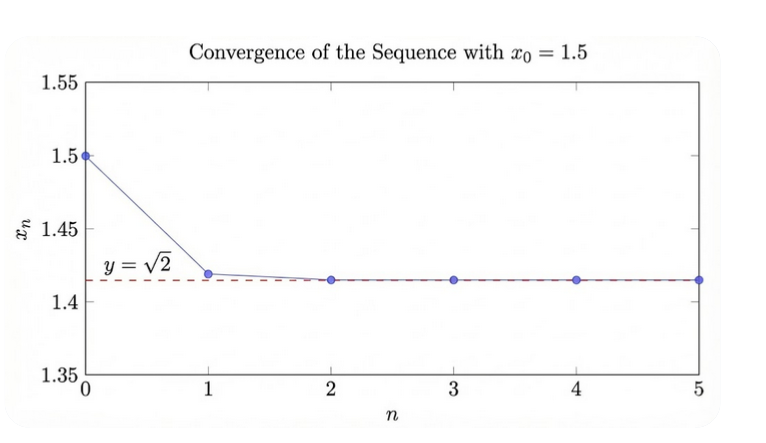
\includegraphics[scale=0.5]{Lectures/images/bounded-1.png}\\
	\end{center}
	Next, to rigorously proof that the limit exists. We can do so by proving this sequence to be monotone and bounded. We can prove that by testing both cases $0<x_0 \le \sqrt{2}$ and $0<x_0<\sqrt{2}$.
	Now, let $(x_n) \rightarrow L$, where $L>0$. Then $(x_{n+1}) \rightarrow L$
	\begin{align*}
		L & = \lim_{n\to \infty} x_{n+1}                                      \\
		  & = \lim_{n \to \infty} \frac{1}{2}\left(x_n + \frac{2}{x_n}\right) \\
		  & = \lim_{n \to \infty} \frac{x_n}{2} + \frac{1}{x_n}               \\
		  & = \frac{L}{2} + \frac{1}{L}
	\end{align*}
	This gives us,
	\begin{align*}
		L                                                             = \frac{L}{2} + \frac{1}{L}
		\implies \frac{L}{2}  =\frac{1}{L}                \implies L  = \sqrt{2}
	\end{align*}
	Hence, the given sequence converges to $\sqrt{2}$.
\end{proof}
\begin{definition}[Convergent sequence; limit of sequence for $\R^n$ Space]
	A sequence $i \rightarrow a_i$ of points $\R^n$ converges to $a \in \R^n$ if
	\[\forall \eps >0, \exists M | m>M \implies |a_m -a| <\eps \]
	We then call $a$, the \emph{limit} of the sequence
\end{definition}
This also holds for vector $a_i$.
\[a_m = [(a_m)_1, (a_m)_2 , \cdots, (a_m)_n] \rightarrow [a_1,a_2, \cdots, a_n]\in \R^n\]
Here, $a_1$ is the convergent point of sequence $(a_m)_1, (a_{m+1})_1, \cdots$. And so on.
\begin{proposition}[Convergence in terms of coordinates]
	A sequence $m \rightarrow a_m$ with $a_m \in \R^n$ convergers to $a$ if and only if each coordinate; \emph{i.e.} for all $1\le j\le n$, the $j$th coordinate  $(a_i)_j)$ of $a_i$ converges to $a_j$, the $j$th coordinate of the limit $a$.
\end{proposition}
\begin{proof}[Proof]
	Let $\| \cdot \|$ denote the standard Euclidean norm in $\mathbb{R}^n$. Recall the definition of sequence convergence: $a_m \to a$ means that for every $\epsilon > 0$, there exists an integer $N$ such that for all $m \ge N$, $\|a_m - a\| < \epsilon$.

	\vspace{1em}
	\noindent\textbf{Forward Direction ($\Rightarrow$):} \\
	Assume $a_m \to a$. We want to show that for any fixed coordinate $j \in \{1, \dots, n\}$, the sequence $(a_m)_j \to a_j$.

	Let $\epsilon > 0$ be given. Because $a_m \to a$, there exists an integer $N$ such that for all $m \ge N$:
	\[
		\|a_m - a\| < \epsilon
	\]
	Observe that the absolute value of any single coordinate difference is bounded by the Euclidean distance:
	\[
		|(a_m)_j - a_j| = \sqrt{((a_m)_j - a_j)^2} \le \sqrt{\sum_{k=1}^n ((a_m)_k - a_k)^2} = \|a_m - a\|
	\]
	Therefore, for all $m \ge N$, we have:
	\[
		|(a_m)_j - a_j| \le \|a_m - a\| < \epsilon
	\]
	Since for any $\epsilon > 0$ we found an $N$ that satisfies this condition, $(a_m)_j \to a_j$ for each $j$.

	\vspace{1em}
	\noindent\textbf{Reverse Direction ($\Leftarrow$):} \\
	Assume that for each $1 \le j \le n$, the coordinate sequence $(a_m)_j \to a_j$. We want to show that the vector sequence $a_m \to a$.

	Let $\epsilon > 0$ be given. By the definition of convergence for each coordinate, there exists an integer $N_j$ such that for all $m \ge N_j$:
	\[
		|(a_m)_j - a_j| < \frac{\epsilon}{\sqrt{n}}
	\]
	We want this to hold for \emph{all} coordinates at the same time, so we choose the largest threshold: let $N = \max\{N_1, N_2, \dots, N_n\}$.

	For any $m \ge N$, $m$ is greater than or equal to every $N_j$, so the inequality $|(a_m)_j - a_j| < \frac{\epsilon}{\sqrt{n}}$ holds for all $j=1, \dots, n$ simultaneously.

	Now, we evaluate the distance between the vectors $a_m$ and $a$ for $m \ge N$:
	\[
		\|a_m - a\| = \sqrt{\sum_{j=1}^n ((a_m)_j - a_j)^2} < \sqrt{\sum_{j=1}^n \left(\frac{\epsilon}{\sqrt{n}}\right)^2}
	\]
	Simplifying the expression under the square root:
	\[
		\|a_m - a\| < \sqrt{\sum_{j=1}^n \frac{\epsilon^2}{n}} = \sqrt{n \cdot \frac{\epsilon^2}{n}} = \sqrt{\epsilon^2} = \epsilon
	\]
	Because for any $\epsilon > 0$ we found an $N$ such that $m \ge N \implies \|a_m - a\| < \epsilon$, the sequence $a_m$ converges to $a$. 
\end{proof}
